\section{Dynamic Range Query Trees}
\begin{frame}
  \begin{center}
    Hand-made Data Structures:\\
    Dynamic Range Query Trees -- Fenwick Tree and Segment Tree\\
    (CP4 2.4.3-4)
  \end{center}
\end{frame}

\subsection{Segment Tree}
\begin{frame}[fragile]
  \frametitle{Range Maximum Query -- RMQ}

  Suppose you have an array of values:
\begin{verbatim}
Value: 18 17 13 19 15 11 20
Index:  0  1  2  3  4  5  6
\end{verbatim}

\bigskip

The \structure{Range Maximum Query} problem asks you to \structure{find
the index with the maximum value} between two indexes:

\begin{itemize}
  \item RMQ(0,0) = 0
  \item RMQ(0,6) = 6
  \item RMQ(1,4) = 3
\end{itemize}

\bigskip

\alert{Naive Method:} loop from $i$ to $j$, find maximum value. $O(nk)$ steps\\
\medskip

But what is the number of {\bf Values (n)} or {\bf Queries (k)} is too big?
\end{frame}

\begin{frame}
  \frametitle{Segment Tree}

  \begin{itemize}
    \item {\bf Basic idea}: Binary tree with the max index in of each subtree.
    \bigskip

    \item {\bf Operation Costs:}
    \begin{itemize}
      \item Creation of the tree: \structure{$O(n)$}
      \item Query of a segment: \structure{$O(\log n)$}
      \item Update of the tree: \structure{$O(\log n)$} \hfill \alert{Important Part}
    \end{itemize}
    \bigskip

    \item There are many implementations. We will show a vector based heap.
  \end{itemize}
\end{frame}

\begin{frame}
  \frametitle{Segment Tree}
  \begin{center}
    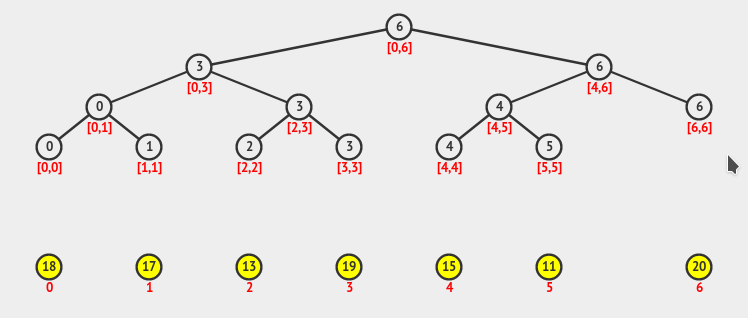
\includegraphics[width=1\textwidth]{img/segment_tree}
  \end{center}

  \bigskip

  Segment Tree animation at VISUALGO: \url{https://visualgo.net/en/segmenttree}
\end{frame}

\begin{frame}[fragile]
  \frametitle{Coding the Segment Tree}
  \framesubtitle{Building the Tree -- add data in array "A", index of biggest value is array "st"}
{\smaller
\begin{block}{}
\begin{verbatim}
typedef vector<int> vi; // vector of ints, we will use this a lot here.

class SegmentTree {     // Object-oriented implementation
private: vi st, A;      // st - Index of biggest, A - value of contents

  int left (int p) { return (p<<1); }     // index of left child;
  int right(int p) { return (p<<1) + 1; } // index of right child;
  void build(int p, int L, int R) {       // Build tree in O(n log n)
    if (L == R)
      st[p] = L;                      // At leaf, largest element is the current.
    else {                            // recursive build the branches.
      build(left(p) , L          , (L+R)/2);   // build left branch
      build(right(p), (L+R)/2 + 1, R      );   // build right branch
      int p1 = st[left(p)], p2 = st[right(p)];
      st[p] = (A[p1] <= A[p2]) ? p1 : p2;      // compare branches.
  } }
\end{verbatim}
\end{block}}
\ppagenote{Segment Tree Code from \url{https://github.com/stevenhalim/cpbook-code}}

\end{frame}

\begin{frame}[fragile]
  \frametitle{Coding the Segment Tree}
  \framesubtitle{Query the Tree -- what is the highest value between i and j?}
{\smaller
\begin{block}{rmq(1, 0, n-1, i, j) -- Query from i to j, bounded by L and R}
\begin{verbatim}
int rmq(int p, int L, int R, int i, int j) // O(log n)
{
  if (i >  R || j <  L)
    return -1;    // query range is outside L/R bounds
  if (L >= i && R <= j)
    return st[p]; // query range is inside L/R bounds

  // compute the highest value in the left and right branches
  int p1 = rmq(left(p) , L        , (L+R)/2, i, j);
  int p2 = rmq(right(p), (L+R)/2+1, R      , i, j);

  if (p1 == -1) return p2;   // left segment outside bounds
  if (p2 == -1) return p1;   // right segment outside bounds
  return (A[p1] <= A[p2]) ? p1 : p2; // return highest of left and right
}
\end{verbatim}
\end{block}}
\end{frame}

\begin{frame}[fragile]
  \frametitle{Coding the Segment Tree}
  \framesubtitle{Update the Tree}

{\smaller
\begin{block}{update(1, 0, n-1, i, v) -- update index i to value v}
\begin{verbatim}
int update(int p, int L, int R, int idx, int new_value) {
  int i = idx, j = idx;
  if (i > R || j < L) return st[p];  // if update ouside interval, return value!

  if (L == i && R == j) {            // if update index matches interval:
    A[i] = new_value;     // update the value array
    return st[p] = L;     // update the leaf index.
  }
  int p1, p2;             // Update left and right branches
  p1=update(left(p) , L        , (L+R)/2, idx, new_value);
  p2=update(right(p), (L+R)/2+1, R      , idx, new_value);

  // Update and return index of current node based on branches.
  return st[p] = (A[p1] <= A[p2]) ? p1 : p2;
}
\end{verbatim}
\end{block}}
\end{frame}
